%Version 3.1 December 2024
%%%%%%%%%%%%%%%%%%%%%%%%%%%%%%%%%%%%%%%%%%%%%%%%%%%%%%%%%%%%%%%%%%%%%%
\documentclass[sn-basic,Numbered,iicol]{sn-jnl}

%%%% Standard Packages
\usepackage{graphicx}%
\usepackage{multirow}%
\usepackage{amsmath,amssymb,amsfonts}%
\usepackage{amsthm}%
\usepackage{mathrsfs}%
\usepackage[title]{appendix}%
\usepackage{xcolor}%
\usepackage{textcomp}%
\usepackage{manyfoot}%
\usepackage{booktabs}%
\usepackage{algorithm}%
\usepackage{algorithmicx}%
\usepackage{algpseudocode}%
\usepackage{listings}%

\theoremstyle{thmstyleone}%
\newtheorem{theorem}{Theorem}%
\newtheorem{proposition}[theorem]{Proposition}%

\theoremstyle{thmstyletwo}%
\newtheorem{example}{Example}%
\newtheorem{remark}{Remark}%

\theoremstyle{thmstylethree}%
\newtheorem{definition}{Definition}%

\raggedbottom

\begin{document}

\title[Temporal Hierarchical Forecast Reconciliation]{Temporal Hierarchical Forecast Reconciliation: Intermediate Aggregation Levels and Forecast Accuracy}

\author*[1]{\fnm{First} \sur{Author}}\email{iauthor@gmail.com}

\affil*[1]{\orgdiv{Department}, \orgname{Organization}, \orgaddress{\street{Street}, \city{City}, \postcode{100190}, \state{State}, \country{Country}}}


%%==================================%%
%% Abstract
%%==================================%%

\abstract{The fundamental goal of the paper is to see whether we can produce more accurate forecasts for a time series at both daily and monthly level by leveraging temporal hierarchical forecast reconciliation. Temporal hierarchical forecast reconciliation is a process where we forecast at different granularities of a single time series at a fixed horizon (e.g.\ daily and weekly for 7 days), then reconcile those forecasts to produce coherent forecasts (e.g.\ the daily forecasts add up to the weekly). Throughout this research, we exclusively evaluate the accuracy of forecasts at two target granularities: daily and monthly. However, we will leverage forecasts at intermediate aggregation levels (e.g.\ weekly) to try and improve the daily and monthly predictions. The objective is to explore how different intermediate aggregation levels can most effectively improve our target forecasts by using reconciliation.}

\keywords{temporal hierarchical forecasting, forecast reconciliation, MinT, time series}

\maketitle

%%==================================%%
%% Introduction
%%==================================%%

\section{Introduction}\label{sec1}

The fundamental goal of the paper is to see whether we can produce more accurate forecasts for a time series at both daily and monthly level by leveraging temporal hierarchical forecast reconciliation. Temporal hierarchical forecast reconciliation is a process where we forecast at different granularities of a single time series at a fixed horizon (e.g.\ daily and weekly for 7 days), then reconcile those forecasts to produce coherent forecasts (e.g.\ the daily forecasts add up to the weekly). Throughout this research, we exclusively evaluate the accuracy of forecasts at two target granularities: daily and monthly. However, we will leverage forecasts at intermediate aggregation levels (e.g.\ weekly) to try and improve the daily and monthly predictions. The objective is to explore how different intermediate aggregation levels can most effectively improve our target forecasts by using reconciliation.

%%==================================%%
%% Related Work
%%==================================%%

\section{Related Work}\label{sec2}

The exact workings of temporal hierarchical forecast reconciliation can be read from \cite{hyndmanforecasting}, and they will not be explained in depth here. Forecast reconciliation is explained in \cite{hyndmanmint}.

%%==================================%%
%% Theorem
%%==================================%%

\section{Theorem for Expansion of Aggregation}\label{sec3}

The theorem which will be proved states the following: \textbf{Adding Intermediate Aggregation Levels Reduces Forecast Error RMSE, at All Aggregation Levels, Under MinT Reconciliation.}

\subsection{Notation and Setup}\label{subsec:notation}

Consider a base period of $n = 28$ days. We observe a scalar time series at daily granularity and wish to forecast at the \textbf{top level} (the 28-day aggregate) and the \textbf{bottom level} (daily).

A \textbf{temporal hierarchy} $\mathcal{H}$ is defined by a set of aggregation levels. Each level $\ell$ specifies how the 28 bottom-level (daily) values are grouped. The relationship between all levels and the bottom level is encoded in a \textbf{summing matrix} $S \in \mathbb{R}^{m \times n}$, where $m$ is the total number of time series across all levels (including the bottom level, so $m \geq n$), and $n = 28$. The matrix satisfies:

\begin{equation}
\mathbf{y} = S \mathbf{b}
\end{equation}

where $\mathbf{b} \in \mathbb{R}^n$ is the vector of true bottom-level values and $\mathbf{y} \in \mathbb{R}^m$ is the full stacked vector of true values at all levels. The bottom $n$ rows of $S$ form the identity $I_n$, and each upper row is a binary (0/1) vector indicating which daily values are summed to form that aggregate.

We produce \textbf{base forecasts} $\hat{\mathbf{y}} \in \mathbb{R}^m$ independently at each level. The base forecast errors are:

\begin{equation}
\hat{\mathbf{e}} = \hat{\mathbf{y}} - \mathbf{y}
\end{equation}

The base forecasts may be \textbf{biased}. We write:

\begin{equation}
\mathbb{E}[\hat{\mathbf{e}}] = \boldsymbol{\delta}
\end{equation}

where $\boldsymbol{\delta} \in \mathbb{R}^m$ is an arbitrary (possibly non-zero) bias vector.

Let $\text{Var}(\hat{\mathbf{e}}) \in \mathbb{R}^{m \times m}$ be the covariance matrix of the base forecast errors. Every covariance matrix is positive semi-definite by construction, since for any \textbf{constant} $\mathbf{x} \in \mathbb{R}^m$ we write the following:

\begin{equation}
\mathbf{x}' \text{Var}(\hat{\mathbf{e}}) \mathbf{x} = \text{Var}(\mathbf{x}'(\hat{\mathbf{e}} - \mathbb{E}[\hat{\mathbf{e}}])) = \text{Var}(\mathbf{x}'(\hat{\mathbf{e}} - \boldsymbol{\delta}))
\end{equation}

To show positive semi-definiteness, we just expand the variance and see that a square is always non-negative:

\begin{equation}
\text{Var}(\mathbf{x}'(\hat{\mathbf{e}} - \mathbb{E}[\hat{\mathbf{e}}])) = \mathbb{E}\left[(\mathbf{x}'(\hat{\mathbf{e}} - \mathbb{E}[\hat{\mathbf{e}}]))^2\right] \geq 0
\end{equation}

For $\text{Var}(\hat{\mathbf{e}})$ to not be positive definite, we would need to show such $\mathbf{x}$ that would make the dot product $\mathbf{x}'(\hat{\mathbf{e}} - \boldsymbol{\delta})$ constant to collapse the variance to zero. The existence of such $\mathbf{x}$ would mean that the $m$ different residuals could be written as a linear combination of other residuals (plus a constant). Because base forecasts are made independently, this is highly unlikely.

\subsection{MinT Reconciliation}\label{subsec:mint}

The MinT (Minimum Trace) reconciled forecast is written and defined as:

\begin{equation}
\tilde{\mathbf{y}} = S \underbrace{(S' \text{Var}(\hat{\mathbf{y}})^{-1} S)^{-1} S' \text{Var}(\hat{\mathbf{y}})^{-1}}_{G} \hat{\mathbf{y}} = S G \hat{\mathbf{y}}
\end{equation}

where $\hat{\mathbf{y}}$ are the independently made, incoherent forecasts, and $\tilde{\mathbf{y}}$ are the coherent forecasts.

This is a \textbf{generalised least squares (GLS)} estimator \cite{hyndmanmint}.

It estimates the leaf/bottom level forecasts by projecting the base forecasts onto the coherent subspace where $\{ S G {\mathbf{y}} = S\mathbf{b} : \mathbf{b} \in \mathbb{R}^n \}$, and then applying the summing matrix.

The reconciled bottom-level forecast is $\tilde{\mathbf{b}} = G \hat{\mathbf{y}}$, and any aggregate level's reconciled forecast is obtained by the appropriate rows of $S \tilde{\mathbf{b}}$.

For simplicity, we can define $\mathbf{P}$ to be

\begin{equation}
\mathbf{P} = \mathbf{S}\mathbf{G}
\end{equation}

\subsubsection{Unbiasedness of MinT}\label{subsubsec:unbiased}

\textbf{Assumption 1 (Unbiasedness).} We assume the base forecasts are unbiased: $\mathbb{E}[\hat{\mathbf{e}}] = \boldsymbol{\delta} = \mathbf{0}$. From here we need to establish that if this assumption is true, then the reconciled forecasts produced from the unbiased base ones, stay unbiased.

We know that MinT reconciliation is an unbiased projection \cite{hyndmanmint} since

\begin{equation}
\mathbf{S}\mathbf{G}\mathbf{S} = \mathbf{S}
\end{equation}

meaning for any coherent forecast $y_c$

\begin{equation}
\mathbf{P}\mathbf{y_c} = \mathbf{y_c}
\end{equation}

We know that the reconciled and base errors can be calculated like:

\begin{align}
\tilde{\mathbf{e}} &= \mathbf{y} - \tilde{\mathbf{y}} \\
\hat{\mathbf{e}} &= \mathbf{y} - \hat{\mathbf{y}}
\end{align}

and if we substitute $\tilde{\mathbf{y}} = \mathbf{P}\hat{\mathbf{y}}$ in the base error formula

\begin{align}
\tilde{\mathbf{e}} &= \mathbf{y} - \mathbf{P}\hat{\mathbf{y}} \nonumber \\
&= \mathbf{y} - \mathbf{P}(\mathbf{y} - \hat{\mathbf{e}}) \nonumber \\
&= \mathbf{y} - \mathbf{P}\mathbf{y} + \mathbf{P}\hat{\mathbf{e}}
\end{align}

Using $\mathbf{P}\mathbf{y} = \mathbf{y}$

\begin{equation}
\tilde{\mathbf{e}} = \mathbf{P}\hat{\mathbf{e}}
\end{equation}

If $\mathbb{E}[\hat{\mathbf{e}}]$ is zero, then

\begin{align}
\mathbb{E}[\tilde{\mathbf{e}}] &= \mathbb{E}[\mathbf{P}\hat{\mathbf{e}}] \nonumber \\
&= \mathbf{P}\mathbb{E}[\hat{\mathbf{e}}] \nonumber \\
&= \mathbf{P}(\mathbf{0}) = \mathbf{0}
\end{align}

Therefore MinT \textbf{preserves unbiasedness}: if the base forecasts are unbiased, so are the reconciled forecasts.

\subsection{Core Theorem}\label{subsec:core}

\subsubsection{Introducing More Levels}\label{subsubsec:morelevels}

The MinT algorithm mathematically formulates forecast reconciliation as a Generalized Least Squares (GLS) regression problem. In this framework, the model is written as:

\begin{equation}
\hat{\mathbf{y}}=\mathbf{S}\mathbf{b}+\mathbf{e}
\end{equation}

where we regress the base forecasts $\hat{\mathbf{y}}$ on the summing matrix $\mathbf{S}$ to estimate the bottom-level coherent forecasts $\mathbf{b}$. If $\mathbf{W} = \text{Var}(\hat{\mathbf{e}})$, then the covariance matrix of the GLS estimator \cite{greeneeconometric} for the bottom level is given by:

\begin{equation}
\text{Var}(\tilde{\mathbf{b}})=(\mathbf{S}'\mathbf{W}^{-1}\mathbf{S})^{-1}
\end{equation}

Let $\mathcal{H}_k$ be a temporal hierarchy with a set of aggregation levels, characterized by the summing matrix $\mathbf{S}_k$ and base forecast covariance $\mathbf{W}_k$. For the sake of the proof, we define $\mathcal{I}_k$ to be the inverse of the bottom level's covariance matrix

\begin{equation}
\mathcal{I}_k=\text{Var}(\tilde{\mathbf{b}})^{-1}=\mathbf{S}_k'\mathbf{W}_k^{-1}\mathbf{S}_k
\end{equation}

When we introduce a new intermediate aggregation level to create hierarchy $\mathcal{H}_{k+1}$, we are appending new observations (base forecasts) to the system. The augmented total covariance matrix $\mathbf{W}_{k+1}$, accounting for potential correlations between the existing and newly added base forecasts, can be written as a block matrix:

\begin{equation}
\mathbf{W}_{k+1}=\begin{bmatrix}\mathbf{W}_k&\mathbf{C}\\\mathbf{C}'&\mathbf{W}_{new}\end{bmatrix}
\end{equation}

where $\mathbf{W}_{new}$ is the variance of the newly added forecasts, and $\mathbf{C}$ is the cross-covariance between the old and new forecasts. The total summing matrix is expanded accordingly:

\begin{equation}
\mathbf{S}_{k+1}=\begin{bmatrix}\mathbf{S}_k\\\mathbf{S}_{new}\end{bmatrix}
\end{equation}

To calculate the new inverse $\mathcal{I}_{k+1}=\mathbf{S}_{k+1}'\mathbf{W}_{k+1}^{-1}\mathbf{S}_{k+1}$, we invert the block covariance matrix $\mathbf{W}_{k+1}$ using the Schur Complement. Let $\mathbf{K}$ be the Schur Complement of $\mathbf{W}_k$ in $\mathbf{W}_{k+1}$:

\begin{equation}
\mathbf{K}=\mathbf{W}_{new}-\mathbf{C}'\mathbf{W}_k^{-1}\mathbf{C}
\end{equation}

Because $\mathbf{W}_{k+1}$ is a positive definite covariance matrix, by the Haynsworth inertia additivity formula, its Schur Complement $\mathbf{K}$ is also positive definite, ensuring $\mathbf{K}^{-1}$ exists and is positive definite \cite{zhangschur}.

Using standard block inversion theorems, the inverse of our total covariance matrix is perfectly defined as:

\begin{equation}
\resizebox{\columnwidth}{!}{$\displaystyle
\mathbf{W}_{k+1}^{-1} = \begin{bmatrix} \mathbf{W}_k^{-1} + \mathbf{W}_k^{-1}\mathbf{C}\mathbf{K}^{-1}\mathbf{C}'\mathbf{W}_k^{-1} & -\mathbf{W}_k^{-1}\mathbf{C}\mathbf{K}^{-1} \\ -\mathbf{K}^{-1}\mathbf{C}'\mathbf{W}_k^{-1} & \mathbf{K}^{-1} \end{bmatrix}
$}
\end{equation}

Now we substitute this block inverse matrix back into our $\mathcal{I}_{k+1}=\mathbf{S}_{k+1}'\mathbf{W}_{k+1}^{-1}\mathbf{S}_{k+1}$ equation:

\begin{equation}
\resizebox{\columnwidth}{!}{$\displaystyle
\mathcal{I}_{k+1} = \begin{bmatrix} \mathbf{S}_k' & \mathbf{S}_{new}' \end{bmatrix} \begin{bmatrix} \mathbf{W}_k^{-1} + \mathbf{W}_k^{-1}\mathbf{C}\mathbf{K}^{-1}\mathbf{C}'\mathbf{W}_k^{-1} & -\mathbf{W}_k^{-1}\mathbf{C}\mathbf{K}^{-1} \\ -\mathbf{K}^{-1}\mathbf{C}'\mathbf{W}_k^{-1} & \mathbf{K}^{-1} \end{bmatrix} \begin{bmatrix} \mathbf{S}_k \\ \mathbf{S}_{new} \end{bmatrix}
$}
\end{equation}

When this matrix multiplication is solved and all the terms are expanded, five distinct terms remain:

\begin{enumerate}
\item $+ \mathbf{S}_k' \mathbf{W}_k^{-1} \mathbf{S}_k$
\item $+ \mathbf{S}_k' \mathbf{W}_k^{-1} \mathbf{C} \mathbf{K}^{-1} \mathbf{C}' \mathbf{W}_k^{-1} \mathbf{S}_k$
\item $- \mathbf{S}_k' \mathbf{W}_k^{-1} \mathbf{C} \mathbf{K}^{-1} \mathbf{S}_{new}$
\item $- \mathbf{S}_{new}' \mathbf{K}^{-1} \mathbf{C}' \mathbf{W}_k^{-1} \mathbf{S}_k$
\item $+ \mathbf{S}_{new}' \mathbf{K}^{-1} \mathbf{S}_{new}$
\end{enumerate}

The first term is exactly $\mathcal{I}_k$. We now rearrange the remaining four terms. Noting that terms 3 and 4 are transposes of each other (since $\mathbf{W}_k$ is symmetric), we can group them as follows:

\begin{align}
&\mathbf{S}_{new}' \mathbf{K}^{-1} \mathbf{S}_{new} - \mathbf{S}_{new}' \mathbf{K}^{-1} \mathbf{C}' \mathbf{W}_k^{-1} \mathbf{S}_k \nonumber \\
&- \mathbf{S}_k' \mathbf{W}_k^{-1} \mathbf{C} \mathbf{K}^{-1} \mathbf{S}_{new} + \mathbf{S}_k' \mathbf{W}_k^{-1} \mathbf{C} \mathbf{K}^{-1} \mathbf{C}' \mathbf{W}_k^{-1} \mathbf{S}_k
\end{align}

Since $\mathbf{W}_k$ is symmetric, so is its inverse, meaning $\mathbf{S}_k'\mathbf{W}_k^{-1}\mathbf{C}$ is the transpose of $\mathbf{C}'\mathbf{W}_k^{-1}\mathbf{S}_k$. We can therefore recognise this as the expansion of a binomial product:

\begin{equation}
(\mathbf{S}_{new}' - \mathbf{S}_k'\mathbf{W}_k^{-1}\mathbf{C}) \; \mathbf{K}^{-1} \; (\mathbf{S}_{new} - \mathbf{C}'\mathbf{W}_k^{-1}\mathbf{S}_k)
\end{equation}

This is a quadratic form $\mathbf{A}'\mathbf{K}^{-1}\mathbf{A}$, where we define:

\begin{equation}
\mathbf{A} = \mathbf{S}_{new} - \mathbf{C}'\mathbf{W}_k^{-1}\mathbf{S}_k
\end{equation}

which is a valid matrix of shape $(m_{new} \times n)$. Therefore, the entire formula collapses into:

\begin{equation}\label{eq:core}
\mathcal{I}_{k+1}=\mathcal{I}_k+\mathbf{A}'\mathbf{K}^{-1}\mathbf{A}
\end{equation}

Because $\mathbf{K}^{-1}$ is positive definite, the quadratic form $\mathbf{A}'\mathbf{K}^{-1}\mathbf{A}$ is mathematically guaranteed to be a PSD matrix \cite{sebermatrix}. Adding a PSD matrix implies an inequality defined by the Loewner partial order:

\begin{equation}
\mathcal{I}_{k+1}\succeq\mathcal{I}_k
\end{equation}

A theorem of the Loewner partial order states that for Hermitian matrices, inversion reverses the inequality \cite{sebermatrix}. A variance matrix $\text{Var}(\tilde{\mathbf{b}})$ is Hermitian because each of its components are real numbers, and it is symmetric. Since $\mathcal{I}$ is defined to be the inverse of $\text{Var}(\tilde{\mathbf{b}})$, it is also Hermitian, therefore the theorem does apply.

\begin{equation}
\mathcal{I}_k^{-1}\succeq\mathcal{I}_{k+1}^{-1}
\end{equation}

\begin{equation}
\text{Var}(\tilde{\mathbf{b}}_k)\succeq\text{Var}(\tilde{\mathbf{b}}_{k+1})
\end{equation}

This proves that incorporating intermediate temporal levels strictly produces a PSD reduction in the covariance of the bottom-level reconciled forecasts, regardless of the correlation structure of the base forecasts.

\subsubsection{Generalization to Aggregations}\label{subsubsec:generalization}

To get the reconciled forecasts across the hierarchy, we apply the summing matrix to the resulting bottom level of the reconciliation: $\tilde{\mathbf{y}}=\mathbf{S}_0\tilde{\mathbf{b}}$. In the research, only aggregation levels which were common across hierarchies were analyzed. Assume that the specific summing matrix to create these common aggregation levels is $\mathbf{S}_0$

\begin{equation}
\text{Var}(\tilde{\mathbf{y}}) = \text{Var}(\mathbf{S}_0\tilde{\mathbf{b}}) = \mathbf{S}_0 \text{Var}(\tilde{\mathbf{b}}) \mathbf{S}_0'
\end{equation}

We have shown that $\text{Var}(\tilde{\mathbf{b}})$ is PSD reduced by incorporating intermediate levels, therefore $\mathbf{\Delta}$ is a PSD matrix given by

\begin{equation}
\mathbf{\Delta} = \text{Var}(\tilde{\mathbf{b}}_k) - \text{Var}(\tilde{\mathbf{b}}_{k+1}) \succeq 0
\end{equation}

We define $\tilde{\mathbf{y}}_k$ and $\tilde{\mathbf{y}}_{k+1}$ to be the reconciled forecasts of the common aggregation levels, from the two hierarchies:

\begin{align}
\tilde{\mathbf{y}}_k &= \mathbf{S}_0 \tilde{\mathbf{b}}_k \\
\tilde{\mathbf{y}}_{k+1} &= \mathbf{S}_0 \tilde{\mathbf{b}}_{k+1}
\end{align}

If we look at the difference of the variances of these common reconciled forecast levels

\begin{align}
\text{Var}(\tilde{\mathbf{y}}_k) - \text{Var}(\tilde{\mathbf{y}}_{k+1}) &= \mathbf{S}_0 \text{Var}(\tilde{\mathbf{b}}_k) \mathbf{S}_0' - \mathbf{S}_0 \text{Var}(\tilde{\mathbf{b}}_{k+1}) \mathbf{S}_0' \nonumber \\
&= \mathbf{S}_0 \left( \text{Var}(\tilde{\mathbf{b}}_k) - \text{Var}(\tilde{\mathbf{b}}_{k+1}) \right) \mathbf{S}_0' \nonumber \\
&= \mathbf{S}_0 \mathbf{\Delta} \mathbf{S}_0'
\end{align}

Because $\mathbf{\Delta}$ is PSD, the quadratic form $\mathbf{S}_0 \mathbf{\Delta} \mathbf{S}_0'$ is also guaranteed to be PSD \cite{sebermatrix}. Therefore, we can write the following.

\begin{equation}
\text{Var}(\tilde{\mathbf{y}}_k) \succeq \text{Var}(\tilde{\mathbf{y}}_{k+1})
\end{equation}

\subsubsection{Application to RMSE}\label{subsubsec:rmse}

Because we have established that $\text{Var}(\tilde{\mathbf{y}}_k)\succeq\text{Var}(\tilde{\mathbf{y}}_{k+1})$, the extracted diagonal elements representing the variance of any specific individual aggregation node $i$ strictly cannot increase:

\begin{equation}
(\text{Var}(\tilde{\mathbf{y}}_k))_{ii}\ge(\text{Var}(\tilde{\mathbf{y}}_{k+1}))_{ii}
\end{equation}

It follows directly that the Root Mean Squared Error (RMSE) for that node cannot increase, as $\text{RMSE}_i=\sqrt{V_{ii}}$. Furthermore, this monotonic non-increase holds true for the Normalised RMSE (NRMSE). Normalisation merely applies a strictly positive scalar divisor $c_i$ (the variance of the training data at that specific granularity) to the RMSE:

\begin{equation}
\text{NRMSE}_i=\frac{\sqrt{V_{ii}}}{c_i}
\end{equation}

Since $c_i$ is a constant derived purely from historical training data and is completely independent of the reconciliation hierarchy, the inequality holds:

\begin{equation}
(\text{NRMSE}_k)_i\ge(\text{NRMSE}_{k+1})_i
\end{equation}

Therefore, we guarantee in theory that adding any intermediate temporal levels to a hierarchy cannot increase the expected NRMSE at any aggregation node.

\subsubsection{In Practice}\label{subsubsec:practice}

What was proven here is that for a single horizon of a base period (i.e.\ 28 days), the NRMSE of individual temporal aggregations do not increase. What was studied in practice is the NRMSE across a greater forecast horizon aggregated across different time series of different properties. While theoretical guarantees show that the expected NRMSE strictly does not increase for any individual aggregation, empirical applications revealed a divergence in summary statistics.

%%==================================%%
%% Experiments
%%==================================%%

\section{Experiments}\label{sec4}

\subsection{Methodology}\label{subsec:methodology}

Experiments of the theorem were done using temporal hierarchies, where the bottom level was daily granularity. These hierarchies are required to be able to use any kind of \textbf{hierarchy level}, defined by a \textbf{summing row}, or to use any kind of \textbf{aggregation level}, defined by a set of summing rows, or a \textbf{subsection of the summing matrix}. An example for a hierarchy level is aggregating every second day into one, and an example for an aggregation level is aggregating every two days, translating to many hierarchy levels of two day aggregations. The ability to use any arbitrary hierarchy level, not only continuous aggregations requires that a \textbf{base period} is defined, which will translate to the width of the summing matrix, determining the limits of the definable temporal aggregations. The base period will be a common period for all aggregations (relative to the granularity of the bottom level).

The base period chosen was 28 days, to be close to the length of a regular month. Since the framework could not allow having proper monthly aggregations with a fixed base period, for the scope of the paper, a month will be exactly 28 days. Because of the nature of the framework, forecast horizons will always be multiples of this base period.

For periodic aggregation levels, the framework fits the base forecast model to the continuous time series defined, to achieve better results, by having the model use the whole continuously aggregated history. Afterwards, the individual forecasts of certain aggregation levels need rearranging for the reconciliation to work. Take the situation where we have monthly, weekly and daily forecasts at a horizon of $3 \times 28$ days: we have 3 monthly forecasts, 12 weekly, and 84 daily ones. Simply these forecasts do not allow us to calculate covariance, since there are different amounts of forecasts. So instead the forecasts are flattened so there will be more virtual variables, with exactly the same amount of samples: 1 row of forecasts will contain the following values as a flat vector: (1 monthly $|$ 4 weekly $|$ 28 daily). For example, this process essentially transforms the 12 weekly forecasts to 3 sets of forecasts for $\text{week}_1, \text{week}_2, \text{week}_3, \text{week}_4$.

Throughout the paper, only AutoETS model is used for producing base forecasts, which are then reconciled by the MinT algorithm, using an estimate of the covariance matrix produced by shrinkage methodology.

\subsection{Dataset}\label{subsec:dataset}

The following requirements are set against datasets.

\begin{itemize}
\item Daily granularity: granularity at at least daily.
\item Has exact date timestamp: this is convenient because we want to aggregate by weekdays and weekends too.
\item Big volume of time series: the effects of theorem shall be tested on average.
\end{itemize}

The datasets used by this paper are the following:

\begin{itemize}
\item Google Web Traffic \cite{kaggle_web_traffic_2017}: In its raw form it has 145k independent time series describing the web traffic of various Wikipedia pages. We took the first 13k time series from this dataset, out of those which contained no missing values.
\end{itemize}

The framework requires a few traits from the input data: the length of the time series shall be a multiple of base period to allow for seamless aggregation of the data as preprocessing. All datasets were transformed this way, finding the first Monday in the time series, and trimming the end so that the number of history days are a multiple of 28.

\begin{itemize}
\item Google Web Traffic: After preprocessing, 784 days of history were left in 13k time series, which equates to 112 weeks, so just over two years.
\end{itemize}

After aggregating the time series and determining the forecast horizon as $h$ days, that amount of days were cut off from the end of each dataset, for validation, leaving the rest for training. Base forecast models are fit at each hierarchy level on appropriate aggregations of the train set. Then by inference we retrieve appropriate amounts of predictions at each hierarchy level, which shall equate to $h$ days of data.

\subsection{Evaluation}\label{subsec:evaluation}

After producing the independent base predictions at each aggregation level and rearranging them, MinT reconciliation is applied to them, producing a set of coherent forecasts. Certain common aggregation levels' base forecasts and the reconciled forecasts are compared with the corresponding validation set, cut off in the preprocessing. These common aggregation levels are the daily, bottom level, and the monthly (i.e.\ 4 weeks), top level aggregations.

The error metric used for comparison is a normalised RMSE metric. The normalisation happens through division by the variance of the specific time series' train set, at the specific aggregation level.

\subsection{Measurements}\label{subsec:measurements}

To study the practical applicability of the theorem, many different temporal hierarchies are evaluated on the datasets. The hierarchies tested are randomly generated by taking samples out of predefined aggregation levels. The exact generation process is as follows:

\begin{itemize}
\item 24 unique aggregation levels are defined. These may result in multiple (but not the same amount of) rows in the summing matrix (e.g.\ weekly aggregation produces 4 rows).
\item Batches of 3 aggregation levels are randomly drawn from this pool sequentially, producing packs of aggregation levels containing 3, 6, 9, 12, 15, 18, 21 unique aggregation levels (24 are not drawn since that is deterministic). Due to the sequential drawing process, each pack is a subset of the next.
\item The common aggregation levels of days and months are appended to the packs of aggregation levels, producing full summing matrices.
\item We call a single occurrence of pack drawing a \textit{sequence} of \textit{Sampled Hierarchy}, which this way will contain 7 different hierarchies, with monotonously increasing amounts of rows in their summing matrix.
\item The amount of aggregation levels used in a single hierarchy is called \textit{height}. Therefore a sequence contains 7 hierarchies with different heights.
\item 10 of these sequences are produced to make 70 different hierarchies.
\end{itemize}

The summing matrix formed by all of the 24 available aggregation levels in the pool is shown in Figure~\ref{fig:full_summing}. An example of the summing matrix for a randomly selected sampled hierarchy is shown in Figure~\ref{fig:sh_summing}.

\begin{figure*}[h]
\centering
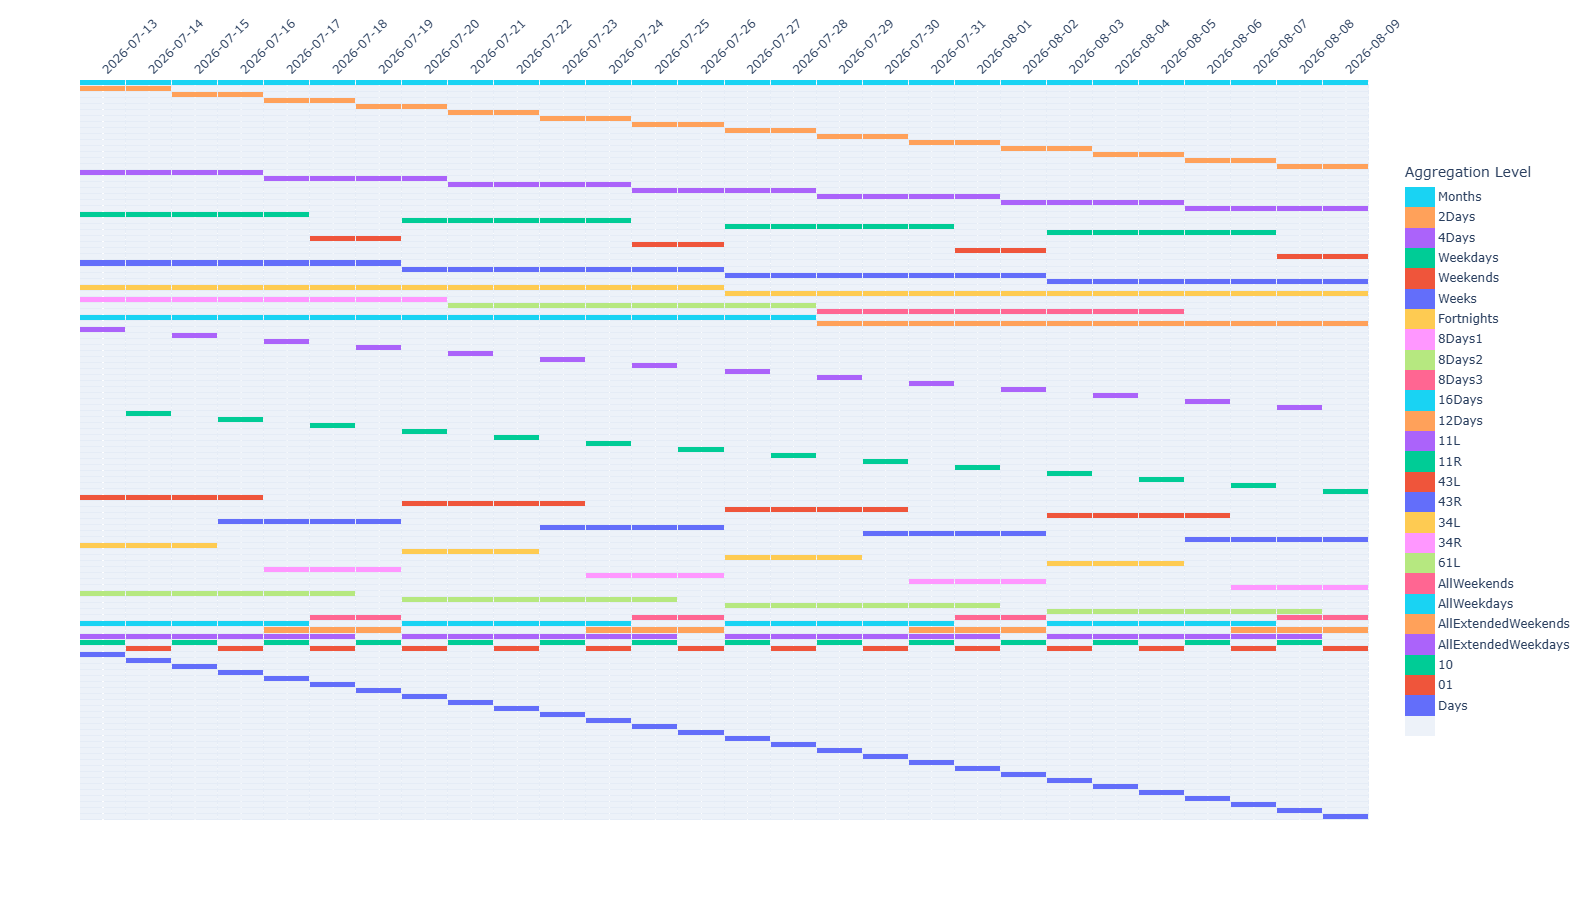
\includegraphics[width=0.9\textwidth]{resources/full_summing.png}
\caption{Summing matrix formed by all available aggregation levels}\label{fig:full_summing}
\end{figure*}

\begin{figure*}[h]
\centering
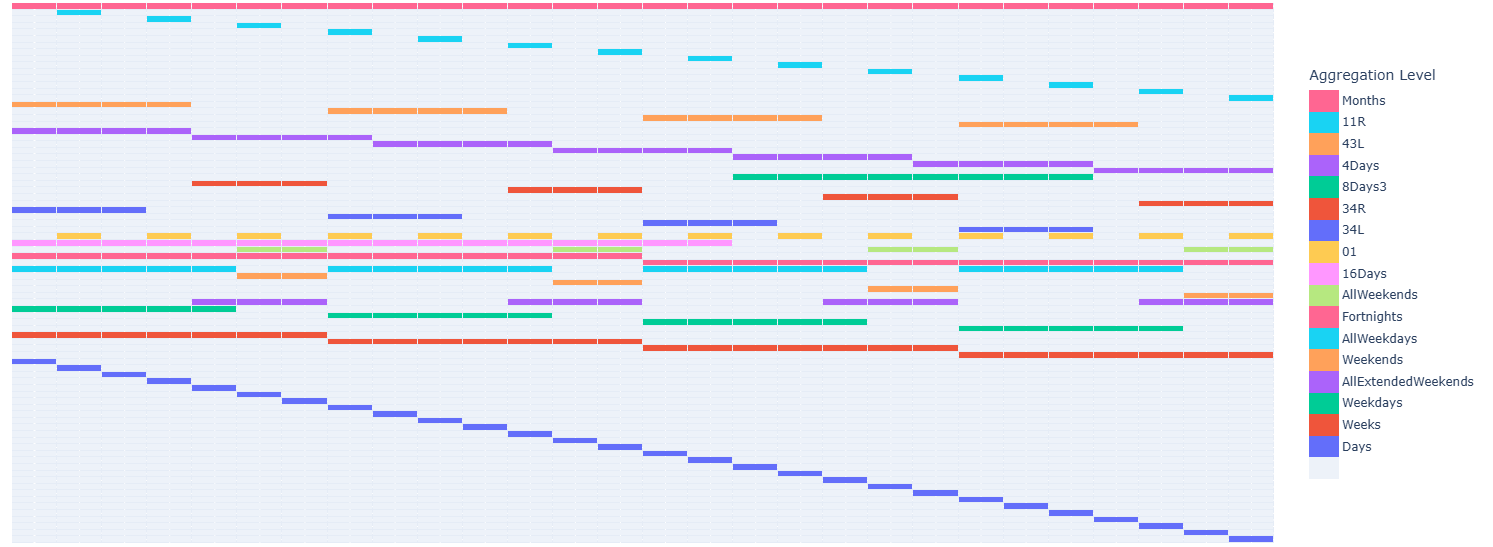
\includegraphics[width=0.9\textwidth]{resources/sh_summing.png}
\caption{Summing matrix of a randomly selected sampled hierarchy with height of 15}\label{fig:sh_summing}
\end{figure*}

For a baseline of comparison, the statistics of the base forecasts, at daily and monthly granularity are seen in Table~\ref{tab:baseline}. The mean of the NRMSE error metric is shown in a raw form, but it is calculated with the top 0.1\% of outliers filtered out.

\begin{table}[h]
\caption{Baseline base forecast error statistics}\label{tab:baseline}
\begin{tabular}{@{}lll@{}}
\toprule
Granularity & Mean NRMSE & Filtered Mean NRMSE \\
\midrule
Months & 1.0514 & 0.9637 \\
Days & 1.2931 & 1.1696 \\
\botrule
\end{tabular}
\end{table}

During the reconciliation process, extreme outliers were frequently introduced, resulting in meaningless mean statistics. This is why only the filtered mean, with the top 0.1\% of values removed are shown with the reconciled forecasts. These mean error metrics produced by individual temporal hierarchies are presented in Table~\ref{fig:day_mean} and Table~\ref{fig:month_mean}. The columns represent different heights (i.e.\ number of intermediate aggregation levels between daily and monthly) of the hierarchies. The rows represent sequences where hierarchies were generated sequentially, by appending more and more aggregation levels to them.

\begin{table*}[h]
\caption{Mean NRMSE error at daily granularity per hierarchy}\label{fig:day_mean}
\begin{tabular*}{\textwidth}{@{\extracolsep\fill}lccccccc}
\toprule
Heights & 3 & 6 & 9 & 12 & 15 & 18 & 21 \\
\midrule
Sequence 0 & 1.1557 & 1.1530 & 1.1536 & 1.1559 & 1.1583 & 1.1675 & 1.1471 \\
Sequence 1 & 1.1768 & 1.1724 & 1.1555 & 1.1534 & 1.1415 & 1.1430 & 1.1515 \\
Sequence 2 & 1.1689 & 1.1644 & 1.1724 & 1.1763 & 1.1719 & 1.1742 & 1.1506 \\
Sequence 3 & 1.1794 & 1.1711 & 1.1533 & 1.1515 & 1.1387 & 1.1443 & 1.1374 \\
Sequence 4 & 1.2149 & 1.1603 & 1.1433 & 1.1468 & 1.1524 & 1.1505 & 1.1418 \\
Sequence 5 & 1.2057 & 1.1612 & 1.1615 & 1.1522 & 1.1459 & 1.1343 & 1.1407 \\
Sequence 6 & 1.1867 & 1.1517 & 1.1508 & 1.1424 & 1.1355 & 1.1447 & 1.1395 \\
Sequence 7 & 1.1629 & 1.1507 & 1.1353 & 1.1341 & 1.1394 & 1.1368 & 1.1405 \\
Sequence 8 & 1.1487 & 1.1414 & 1.1370 & 1.1378 & 1.1331 & 1.1372 & 1.1375 \\
Sequence 9 & 1.1974 & 1.1738 & 1.1542 & 1.1523 & 1.1567 & 1.1352 & 1.1410 \\
\midrule
Mean & 1.1797 & 1.1600 & 1.1517 & 1.1503 & 1.1473 & 1.1468 & 1.1428 \\
Std & 0.0205 & 0.0102 & 0.0105 & 0.0111 & 0.0116 & 0.0130 & 0.0049 \\
\botrule
\end{tabular*}
\end{table*}

\begin{table*}[h]
\caption{Mean NRMSE error at monthly granularity per hierarchy}\label{fig:month_mean}
\begin{tabular*}{\textwidth}{@{\extracolsep\fill}lccccccc}
\toprule
Heights & 3 & 6 & 9 & 12 & 15 & 18 & 21 \\
\midrule
Sequence 0 & 1.2745 & 1.2391 & 1.2297 & 1.2163 & 1.1994 & 1.2029 & 1.1873 \\
Sequence 1 & 1.2764 & 1.2582 & 1.2276 & 1.2019 & 1.1794 & 1.1751 & 1.1706 \\
Sequence 2 & 1.2720 & 1.2458 & 1.2305 & 1.2310 & 1.2151 & 1.2010 & 1.1799 \\
Sequence 3 & 1.3069 & 1.2583 & 1.2212 & 1.2060 & 1.1908 & 1.1928 & 1.1720 \\
Sequence 4 & 1.3484 & 1.2593 & 1.2065 & 1.1943 & 1.1921 & 1.1866 & 1.1679 \\
Sequence 5 & 1.3487 & 1.2581 & 1.2230 & 1.1930 & 1.1857 & 1.1718 & 1.1721 \\
Sequence 6 & 1.3204 & 1.2257 & 1.2079 & 1.1891 & 1.1815 & 1.1751 & 1.1694 \\
Sequence 7 & 1.2963 & 1.2301 & 1.2040 & 1.1840 & 1.1784 & 1.1684 & 1.1685 \\
Sequence 8 & 1.2938 & 1.2204 & 1.2030 & 1.1996 & 1.1836 & 1.1755 & 1.1722 \\
Sequence 9 & 1.3104 & 1.2565 & 1.2199 & 1.1958 & 1.1889 & 1.1760 & 1.1733 \\
\midrule
Mean & 1.3048 & 1.2452 & 1.2173 & 1.2011 & 1.1895 & 1.1825 & 1.1733 \\
Std & 0.0266 & 0.0145 & 0.0103 & 0.0131 & 0.0105 & 0.0118 & 0.0057 \\
\botrule
\end{tabular*}
\end{table*}

It is apparent from Table~\ref{fig:day_mean} and Table~\ref{fig:month_mean} how in this setup, the error metrics could only improve compared to the baseline at daily granularity. In both cases, the theorem's effects are apparent.

We can look at the percentage of how many height increase steps follow the theorem per each sequence (Table~\ref{tab:conformism}). For example, a value of 50\% for a sequence would mean that during the aggregation level drawing process, exactly half of the error statistic values produced by the draws followed the theorem, resulting in lower mean NRMSE, than the last.

\begin{table*}[h]
\caption{Theorem conformism percentage per sequence}\label{tab:conformism}
\begin{tabular*}{\textwidth}{@{\extracolsep\fill}lcccccccccc}
\toprule
Sequence & 0 & 1 & 2 & 3 & 4 & 5 & 6 & 7 & 8 & 9 \\
\midrule
Monthly (\%) & 83.3 & 100 & 83.3 & 83.3 & 100 & 83.3 & 100 & 83.3 & 100 & 100 \\
Daily (\%) & 33.3 & 66.7 & 50.0 & 83.3 & 66.7 & 66.7 & 83.3 & 66.7 & 50.0 & 66.7 \\
\botrule
\end{tabular*}
\end{table*}

The monthly results suggest that there were five sequences where there was only a single step which was inconsistent with the trend. The daily data shows a weaker adherence to the theorem, though the trend still holds for more than half the aggregation level increase steps.

%%==================================%%
%% Conclusion
%%==================================%%

\section{Conclusion}\label{sec5}

We have proven that under MinT reconciliation with unbiased base forecasts, adding intermediate temporal aggregation levels to a hierarchy is guaranteed to produce a positive semi-definite reduction in the covariance of reconciled forecasts at all levels. This translates directly to a non-increasing NRMSE at every aggregation node.

Empirical experiments on the Google Web Traffic dataset with 70 randomly generated temporal hierarchies showed that this theoretical guarantee largely holds in practice for summary statistics, with monthly forecasts conforming strongly (83--100\% of steps) and daily forecasts showing weaker but still majority adherence (33--83\% of steps). The gap between theory and practice is attributed to the aggregation of results across multiple time series and longer forecast horizons than a single base period.

\backmatter

\bmhead{Acknowledgements}

Not applicable.

\section*{Declarations}

\begin{itemize}
\item Funding: Not applicable
\item Conflict of interest/Competing interests: Not applicable
\item Data availability: The Google Web Traffic dataset is publicly available on Kaggle.
\item Code availability: Not applicable
\end{itemize}

%%===========================================================================================%%

\bibliography{sn-bibliography}% common bib file

\end{document}
